\documentclass[aspectratio=169,10pt]{beamer}
\usepackage[utf8]{inputenc}
\usepackage[T1]{fontenc}
\usepackage[spanish,es-nodecimaldot,es-noshorthands]{babel}
\usepackage{amsmath,amssymb}
\usepackage{booktabs}
\usepackage{graphicx}
\graphicspath{{figuras/}}

\usetheme{default}
\definecolor{tinta}{HTML}{1D2433}
\definecolor{azul}{HTML}{2F6F9F}
\definecolor{naranja}{HTML}{D1603D}
\setbeamercolor{frametitle}{bg=tinta,fg=white}
\setbeamercolor{title}{fg=tinta}
\setbeamercolor{structure}{fg=azul}
\setbeamercolor{alerted text}{fg=naranja}
\setbeamertemplate{navigation symbols}{}
\setbeamertemplate{frametitle}{\nointerlineskip\begin{beamercolorbox}[wd=\paperwidth,ht=2.6ex,dp=1.2ex,leftskip=1em]{frametitle}\usebeamerfont{frametitle}\insertframetitle\end{beamercolorbox}}
\setbeamertemplate{footline}{\hfill\scriptsize\color{gray}\insertframenumber/\inserttotalframenumber\hspace{1em}\vspace{0.6em}}
\newcommand{\dato}[2]{\begin{minipage}{0.3\textwidth}\centering{\Huge\color{naranja}\textbf{#1}}\\[0.3em]\small #2\end{minipage}}

\title{Multicolinealidad en la ecuación de salarios de Mincer}
\subtitle{Regresión simple y múltiple, inferencia y diagnóstico con datos reales}
\author{Ximena Lara}
\institute{Fundamentos de Econometría}
\date{Noviembre 2026}

\begin{document}

\begin{frame}
\titlepage
\end{frame}

\begin{frame}{Contenido}
\begin{columns}[T]
\column{0.5\textwidth}
\begin{enumerate}
\item Datos y pregunta
\item Regresión lineal simple
\item 4.1 Supuestos
\item 4.2 Parámetros y formas funcionales
\item 4.3 Prueba F y ANOVA
\item 4.4 Dummies e interacciones
\item 4.5 $R^2$ y $\bar R^2$
\item 4.6 Precios hedónicos
\item 4.7 Modelos no anidados
\item 4.8 Regresión cuantílica
\end{enumerate}
\column{0.5\textwidth}
\begin{enumerate}\setcounter{enumi}{10}
\item 4.9 Aplicaciones financieras
\item Multicolinealidad: diagnóstico
\item Multicolinealidad: corrección
\item MANOVA
\item 5.1--5.2 Residuos
\item 5.3--5.6 Heteroscedasticidad
\item 5.7--5.10 Autocorrelación
\item 5.11--5.12 Dinámica y rezagos
\item 5.13 Jarque--Bera
\item Predicción y conclusiones
\end{enumerate}
\end{columns}
\end{frame}

\section{Datos}
\begin{frame}{Pregunta y datos}
\textbf{¿Cuánto aumenta el salario un año más de educación?} Los controles (experiencia, edad, habilidad,
escolaridad de los padres) están muy correlacionados $\Rightarrow$ \alert{multicolinealidad}.
\[
\ln w_i=\beta_0+\beta_1 educ_i+\beta_2 exper_i+\beta_3 exper_i^2+\beta_4 tenure_i+\dots+\varepsilon_i
\]
\centering\small
\begin{tabular}{lll}
\toprule
Base & Fuente & Uso \\
\midrule
wage2 & Wooldridge (NLS 1980), $n=722$ & Base principal \\
hprice1 & Wooldridge, 88 casas & 4.6 Hedónicos \\
stocks & Plotly, semanal 2018--2019 & 4.9 Finanzas \\
macrodata & statsmodels, 1959--2009 & 5.7--5.12 Series de tiempo \\
\bottomrule
\end{tabular}
\end{frame}

\section{Regresión lineal simple}
\begin{frame}{Regresión lineal simple: $\ln w_i=\beta_0+\beta_1 educ_i+u_i$}
\begin{columns}[T]
\column{0.42\textwidth}\small
\[\hat\beta_1=\frac{S_{xy}}{S_{xx}}=\frac{211.41}{3607.2}=0.0586\]
\[\hat\beta_0=\bar y-\hat\beta_1\bar x=5.9991\]
\begin{itemize}
\item $se(\hat\beta_1)=0.00664$, \ $t=8.83$
\item IC 95\%: $[0.0456,\ 0.0716]$
\item $R^2=\hat\rho_{xy}^2=0.0977$
\item $F_{1,720}=t^2=77.97$
\item $\sum\hat u_i=0$, \ $\sum x_i\hat u_i=0$
\end{itemize}
\column{0.58\textwidth}
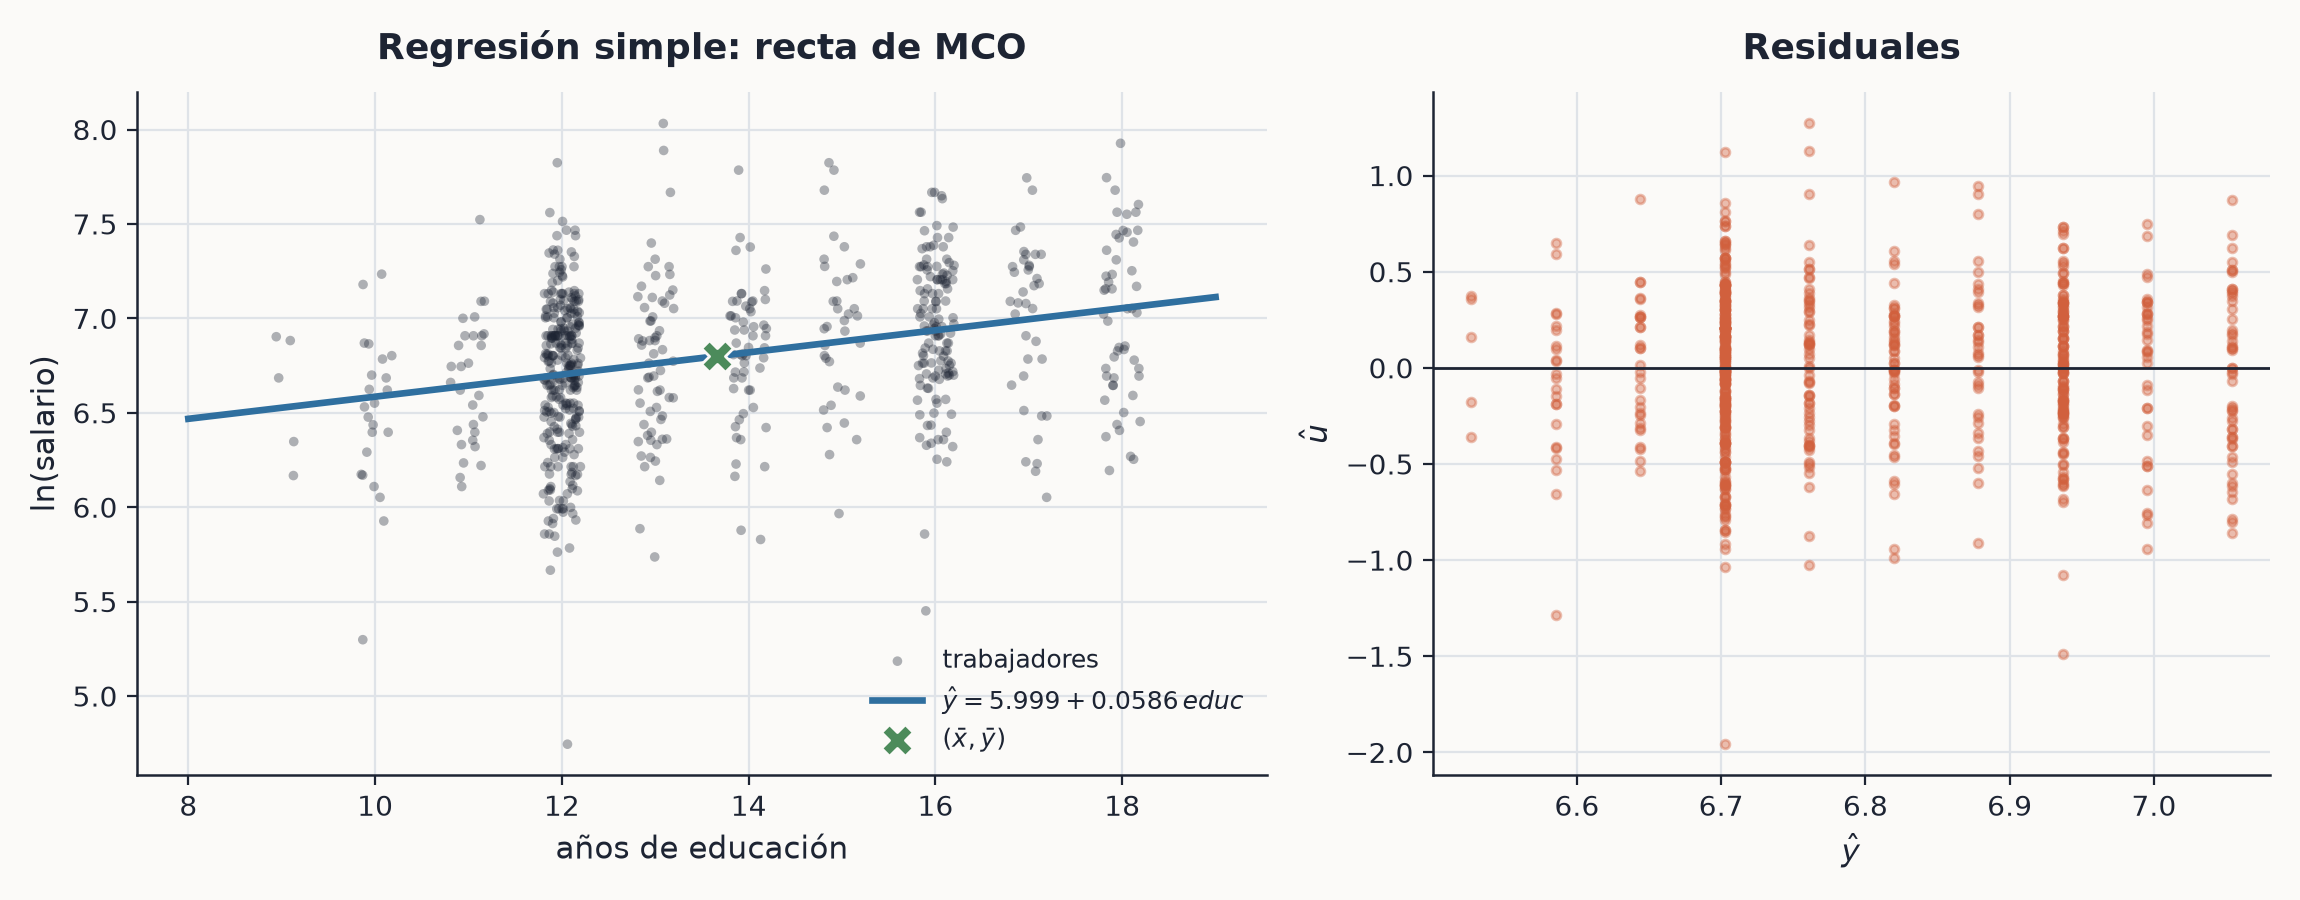
\includegraphics[width=\linewidth]{simple_recta}\\[0.3em]
\small +1 año $\Rightarrow$ \alert{+5.9\%} de salario (exacto 6.0\%), pero la educación sola explica sólo el 9.8\%.
\end{columns}
\end{frame}

\begin{frame}{Regresión simple: propiedades}
\begin{columns}[T]
\column{0.45\textwidth}
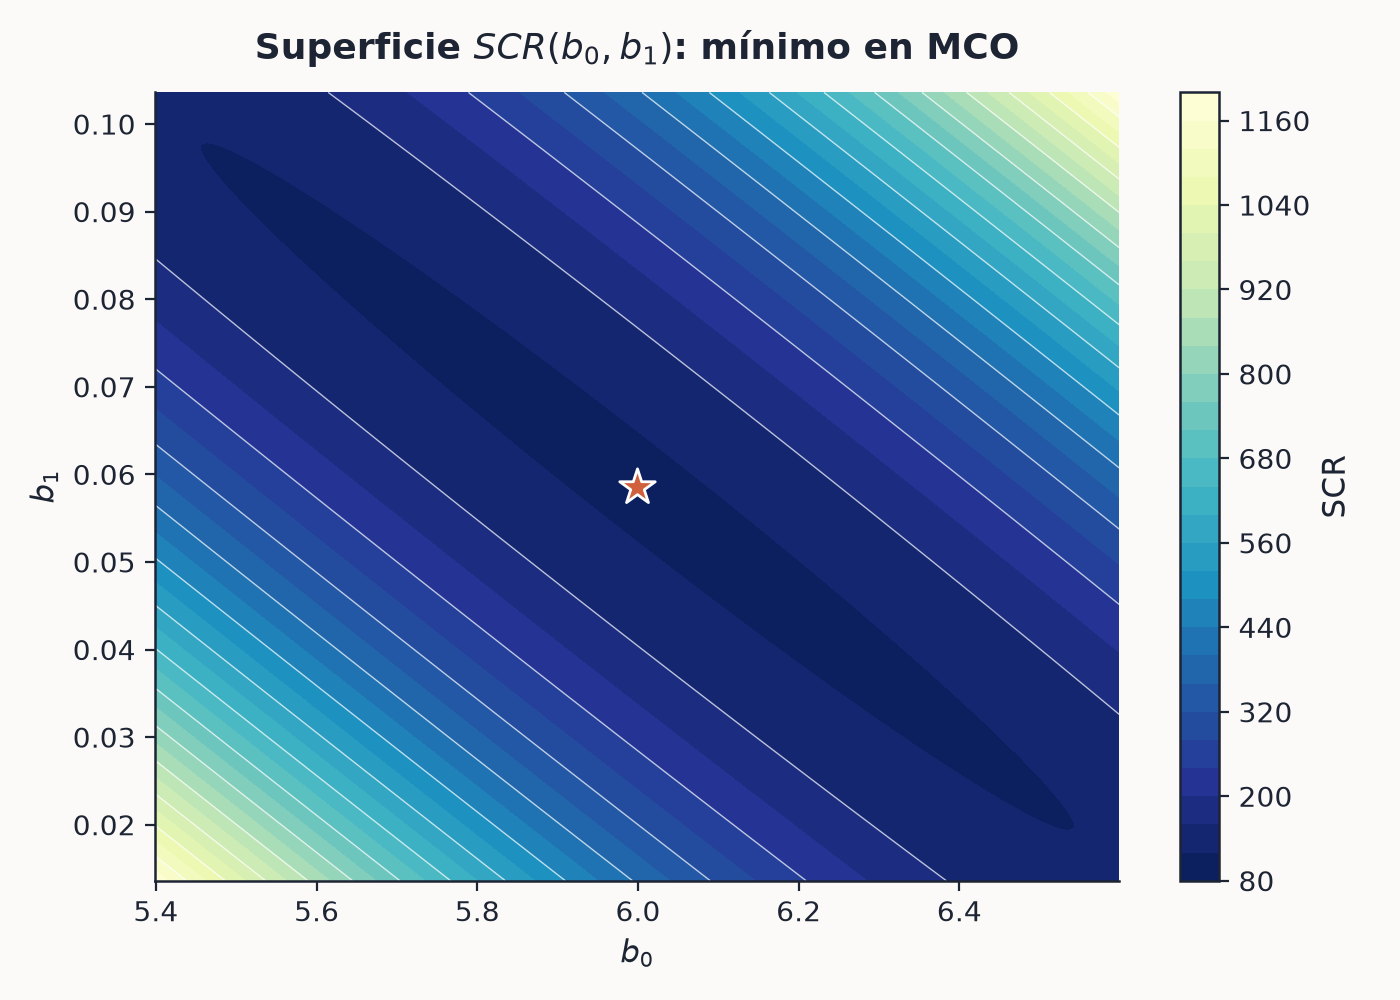
\includegraphics[width=\linewidth]{simple_scr}
\column{0.55\textwidth}\small
\begin{itemize}
\item Superficie $SCR(b_0,b_1)$: mínimo en MCO. Elipse alargada porque $\mathrm{corr}(\hat\beta_0,\hat\beta_1)=-0.987$ ($\bar x$ lejos de 0).
\item Dummy: en $\ln w\sim urban$, $\hat\beta_0=6.6521=\bar y_{rural}$ y $\hat\beta_1=0.2048=\bar y_{urb}-\bar y_{rural}$.
\item Reescalar $x'=12\,educ$, $y'=w/1000$: la pendiente se multiplica por $c/b$ y $R^2$ no cambia.
\item Sin las 10 observaciones más influyentes (Cook): $\hat\beta_1$ pasa de 0.0586 a 0.0601.
\item Gauss--Markov (5{,}000 simulaciones): $\mathrm{Var}_{MCO}=4.4\times10^{-5}<\mathrm{Var}_{alt}=8.7\times10^{-5}$.
\end{itemize}
\end{columns}
\end{frame}

\section{4.1--4.3}
\begin{frame}{4.1 Supuestos del modelo de regresión lineal múltiple}
\centering\small
\begin{tabular}{lll}
\toprule
Supuesto & ¿Se cumple? & Evidencia \\
\midrule
Linealidad en parámetros & Sí & RESET $p=0.43$ \\
Rango completo & Falla con $age-educ-6$ & rango 3 de 4 \\
$E(\varepsilon|X)=0$ & Dudoso sin habilidad & $\hat\beta_{educ}$: 0.078 $\to$ 0.041 \\
Homoscedasticidad & Rechazada (leve) & BP $p=0.022$ \\
No autocorrelación & No aplica (corte transversal) & DW depende del orden \\
Normalidad & Rechazada; $n$ grande & JB $=114$ \\
\bottomrule
\end{tabular}
\end{frame}

\begin{frame}{4.2 Parámetros: formas funcionales e interpretación ceteris paribus}
\centering\small
\begin{tabular}{llrl}
\toprule
Forma & Modelo & $\hat\beta$ & Lectura \\
\midrule
Nivel--nivel & $w=\beta_0+\beta_1 educ$ & 58.59 & +1 año $\to$ +58.6 USD/mes \\
Log--nivel & $\ln w=\beta_0+\beta_1 educ$ & 0.0586 & +1 año $\to$ +5.9\% \\
Nivel--log & $w=\beta_0+\beta_1\ln educ$ & 816.28 & +1\% $\to$ +8.16 USD \\
Log--log & $\ln w=\beta_0+\beta_1\ln educ$ & 0.821 & elasticidad 0.82 \\
\bottomrule
\end{tabular}
\vspace{0.8em}
\begin{itemize}\small
\item Cada $\beta_j$ es un efecto parcial: compara trabajadores iguales en las demás regresoras.
\item Si dos regresoras casi siempre se mueven juntas, hay poca información para separar sus efectos.
\end{itemize}
\end{frame}

\begin{frame}{4.3 ANOVA y prueba F global}
\[F=\frac{(SSR_R-SSR_{NR})/q}{SSR_{NR}/(n-k-1)}\overset{H_0}{\sim}F_{q,\,n-k-1}\]
\centering\small
\begin{tabular}{lrrr}
\toprule
Fuente & SC & gl & CM \\
\midrule
Explicada (SSE) & 33.510 & 13 & 2.5777 \\
Residual (SSR) & 93.302 & 708 & 0.1318 \\
Total (SST) & 126.812 & 721 &  \\
\bottomrule
\end{tabular}
\vspace{0.6em}

$F=19.56>F_{0.05;\,13,\,708}=1.734$ $\Rightarrow$ el modelo es globalmente significativo.
\end{frame}

\begin{frame}{4.3 Pruebas F de restricciones}
\centering\scriptsize
\begin{tabular}{lrrrrl}
\toprule
$H_0$ & $q$ & $F$ & $F_{0.05}$ & $p$ & Decisión \\
\midrule
$\beta_{IQ}=\beta_{KWW}=\beta_{meduc}=\beta_{feduc}=0$ & 4 & 5.416 & 2.385 & $<0.001$ & Rechaza \\
$\beta_{exper}=\beta_{exper^2}=\beta_{age}=0$ & 3 & 5.475 & 2.617 & 0.001 & Rechaza \\
$\beta_{south}=\beta_{urban}=0$ & 2 & 21.282 & 3.008 & $<0.001$ & Rechaza \\
$\beta_{age}=0$ & 1 & 1.110 & 3.855 & 0.293 & No rechaza \\
$\beta_{meduc}=\beta_{feduc}$ & 1 & 0.032 & 3.855 & 0.857 & No rechaza \\
\bottomrule
\end{tabular}
\vspace{0.5em}

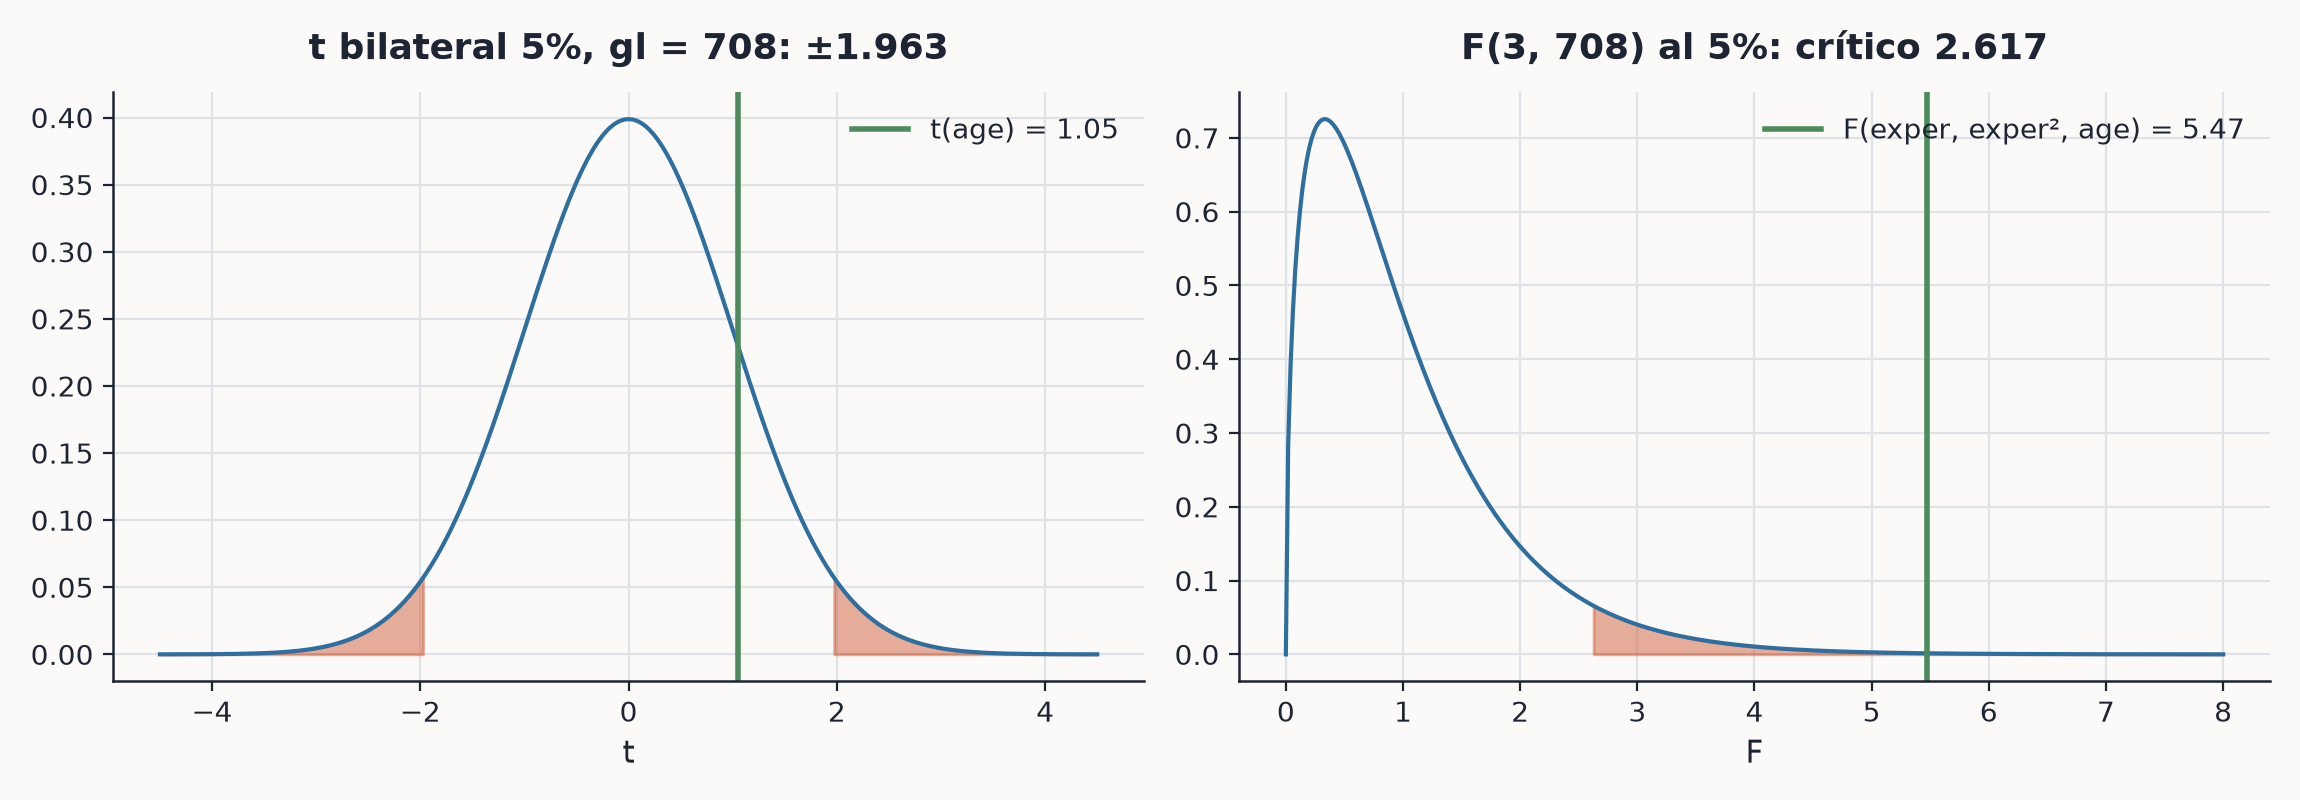
\includegraphics[height=0.42\textheight]{regiones_rechazo}

\small $age$ sola no es significativa ($F=t^2=1.11$), pero $\{exper, exper^2, age\}$ \alert{sí lo es en conjunto}.
\end{frame}

\section{4.4--4.7}
\begin{frame}{4.4 Dummies e interacciones}
\[\ln w=\beta_0+\beta_1 educ+\dots+\delta\,black+\gamma\,(educ\times black)+\varepsilon\]
\begin{itemize}
\item Bases: no casado, no negro, fuera del sur, rural. Efecto exacto $100(e^{\beta}-1)$.
\item Casado: \alert{+21.9\%}; urbano: \alert{+20.8\%}; sur: $-$7.1\%.
\item Pendiente de educación: grupo base 0.0541; negros $\beta_1+\gamma=0.0296$ ($\gamma$: $p=0.34$).
\item $\delta$ sola es la diferencia sólo si $educ=0$; con 12 años: $\delta+12\gamma=$-$0.090$.
\item \textbf{Trampa de las dummies}: constante $+$ urban $+$ rural $\Rightarrow$ rango 3 de 4 (colinealidad perfecta).
\end{itemize}
\end{frame}

\begin{frame}{4.5 $R^2$ y $R^2$ ajustada \quad\textbar\quad 4.6 Precios hedónicos}
\begin{columns}[T]
\column{0.45\textwidth}\centering\small
\begin{tabular}{lrrr}
\toprule
Modelo & $k$ & $R^2$ & $\bar R^2$ \\
\midrule
Completo & 13 & 0.2778 & 0.2633 \\
+ sibs & 14 & 0.2780 & 0.2624 \\
+ sibs + brthord & 15 & 0.2802 & 0.2635 \\
+ hours & 14 & 0.2897 & 0.2743 \\
\bottomrule
\end{tabular}\\[0.5em]
\raggedright Agregar \texttt{sibs} sube $R^2$ pero baja $\bar R^2$.
\column{0.55\textwidth}\small
\textbf{hprice1} (88 casas):
\[\ln P=\beta_0+\beta_1\ln lot+\beta_2\ln sqrft+\beta_3 bdrms+\beta_4 colonial\]
\begin{itemize}
\item Elasticidad precio--superficie: 0.707 ($p<0.001$).
\item Recámaras: 0.027 ($p=0.35$): con la misma superficie no agregan valor.
\item Con el avalúo: VIF de $\ln sqrft$ 1.48 $\to$ 5.10; $se$ 0.093 $\to$ 0.138.
\end{itemize}
\end{columns}
\end{frame}

\begin{frame}{4.7 Modelos no anidados}
A: controles $+$ habilidad (IQ, KWW) \qquad B: controles $+$ familia (meduc, feduc)
\vspace{0.5em}
\centering\small
\begin{tabular}{lll}
\toprule
 & A (habilidad) & B (familia) \\
\midrule
AIC & 599.7 & 609.1 \\
BIC & 650.1 & 659.5 \\
$\bar R^2$ & 0.2476 & 0.2378 \\
Prueba J & $\hat y_B$ en A: $t=2.21$, $p=0.028$ & $\hat y_A$ en B: $t=3.77$, $p<0.001$ \\
\bottomrule
\end{tabular}
\vspace{0.6em}
\begin{itemize}\small
\item AIC, BIC y $\bar R^2$ prefieren A.
\item La prueba J de Davidson--MacKinnon rechaza en \alert{ambas} direcciones: ninguno abarca al otro $\Rightarrow$ combinarlos\ldots\ y aparece la multicolinealidad.
\end{itemize}
\end{frame}

\section{4.8--4.9}
\begin{frame}{4.8 Regresión cuantílica: $Q_\tau(\ln w\mid X)=X'\beta_\tau$}
\begin{columns}[T]
\column{0.55\textwidth}
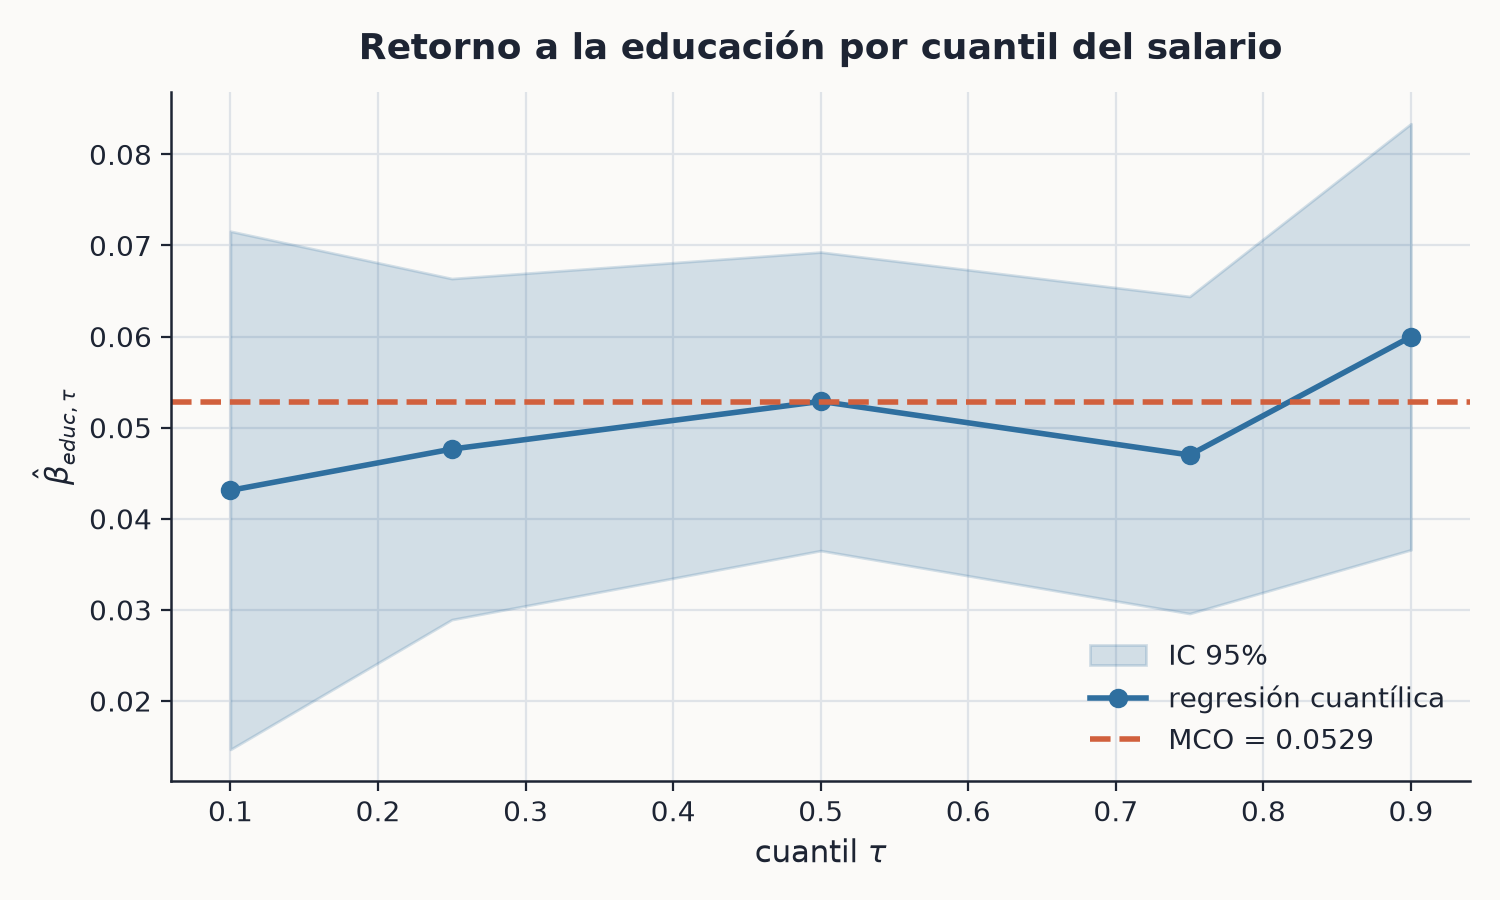
\includegraphics[width=\linewidth]{cuantilica}
\column{0.45\textwidth}\centering\small
\begin{tabular}{rrrr}
\toprule
$\tau$ & $\hat\beta_{educ}$ & ee & IC 95\% \\
\midrule
0.1 & 0.0431 & 0.0145 & [0.015, 0.072] \\
0.25 & 0.0476 & 0.0095 & [0.029, 0.066] \\
0.5 & 0.0529 & 0.0083 & [0.037, 0.069] \\
0.75 & 0.0470 & 0.0089 & [0.030, 0.064] \\
0.9 & 0.0600 & 0.0119 & [0.037, 0.083] \\
\bottomrule
\end{tabular}\\[0.6em]
\raggedright MCO: 0.0529. El retorno va de 4.3\% a 6.0\%, pero los IC se traslapan: heterogeneidad moderada.
\end{columns}
\end{frame}

\begin{frame}{4.9 Aplicaciones financieras: beta de mercado de AAPL}
\begin{columns}[T]
\column{0.55\textwidth}
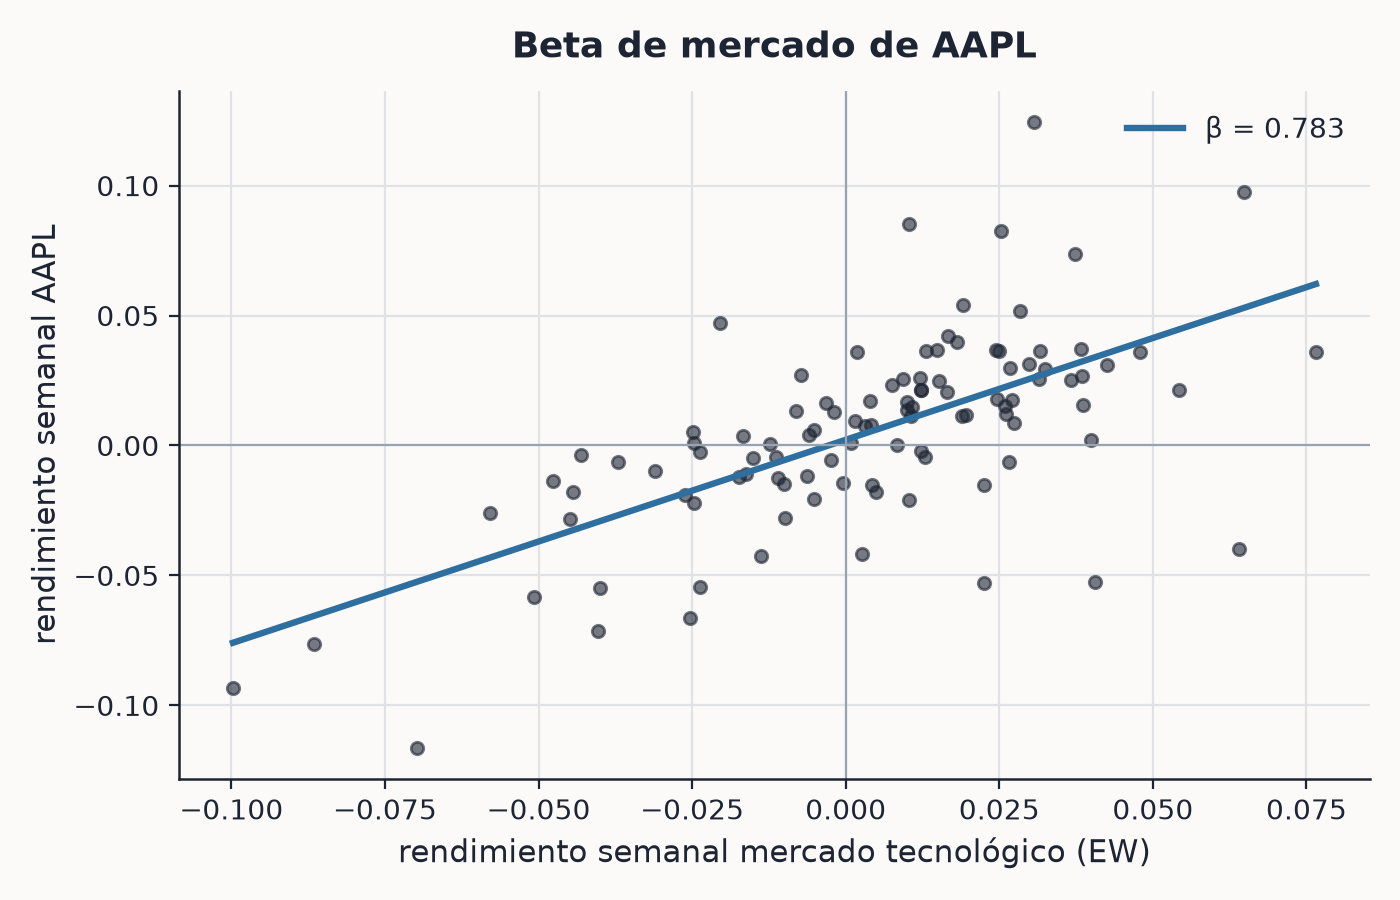
\includegraphics[width=\linewidth]{capm}
\column{0.45\textwidth}\small
Rendimientos log semanales 2018--2019, $n=104$.
\begin{itemize}
\item $\hat\beta=0.783$, IC 95\% $[0.600,\ 0.966]$
\item $\hat\alpha=0.0022$ ($p=0.44$): sin alfa
\item BP $p=0.098$; BG(4) $p=0.82$
\item JB $p<0.001$: colas pesadas
\item AAPL $\sim$ MSFT $+$ AMZN $+$ GOOG: $F=14.62$ ($p<0.001$), pero sólo MSFT es significativa: acciones correlacionadas.
\end{itemize}
\end{columns}
\end{frame}

\section{Multicolinealidad}
\begin{frame}{Multicolinealidad: perfecta vs imperfecta}
\textbf{Perfecta:} experiencia potencial $pexper=age-educ-6$. Con constante, $educ$, $age$ y $pexper$:
rango$(X)=3<4$, $\kappa(X'X)\approx 9.6\times10^{16}$ $\Rightarrow$ $(X'X)^{-1}$ no existe.
\vspace{1em}

\textbf{Imperfecta} (modelo completo, 13 regresores):
\vspace{0.6em}

\centering
\dato{24}{VIF máximo ($exper^2$)}\hfill
\dato{77}{número de condición (BKW) $>30$}\hfill
\dato{4140}{$\chi^2$ Farrar--Glauber (crítico 99.6)}
\vspace{1em}

\raggedright\small
$t$ individuales: $exper$ 1.09, $exper^2$ $-$0.22, $age$ 1.05 \ldots\ pero $F$ conjunta $=5.47$ ($p=0.001$).
\end{frame}

\begin{frame}{Correlaciones, VIF, tolerancia y regla de Klein}
\begin{columns}[T]
\column{0.5\textwidth}
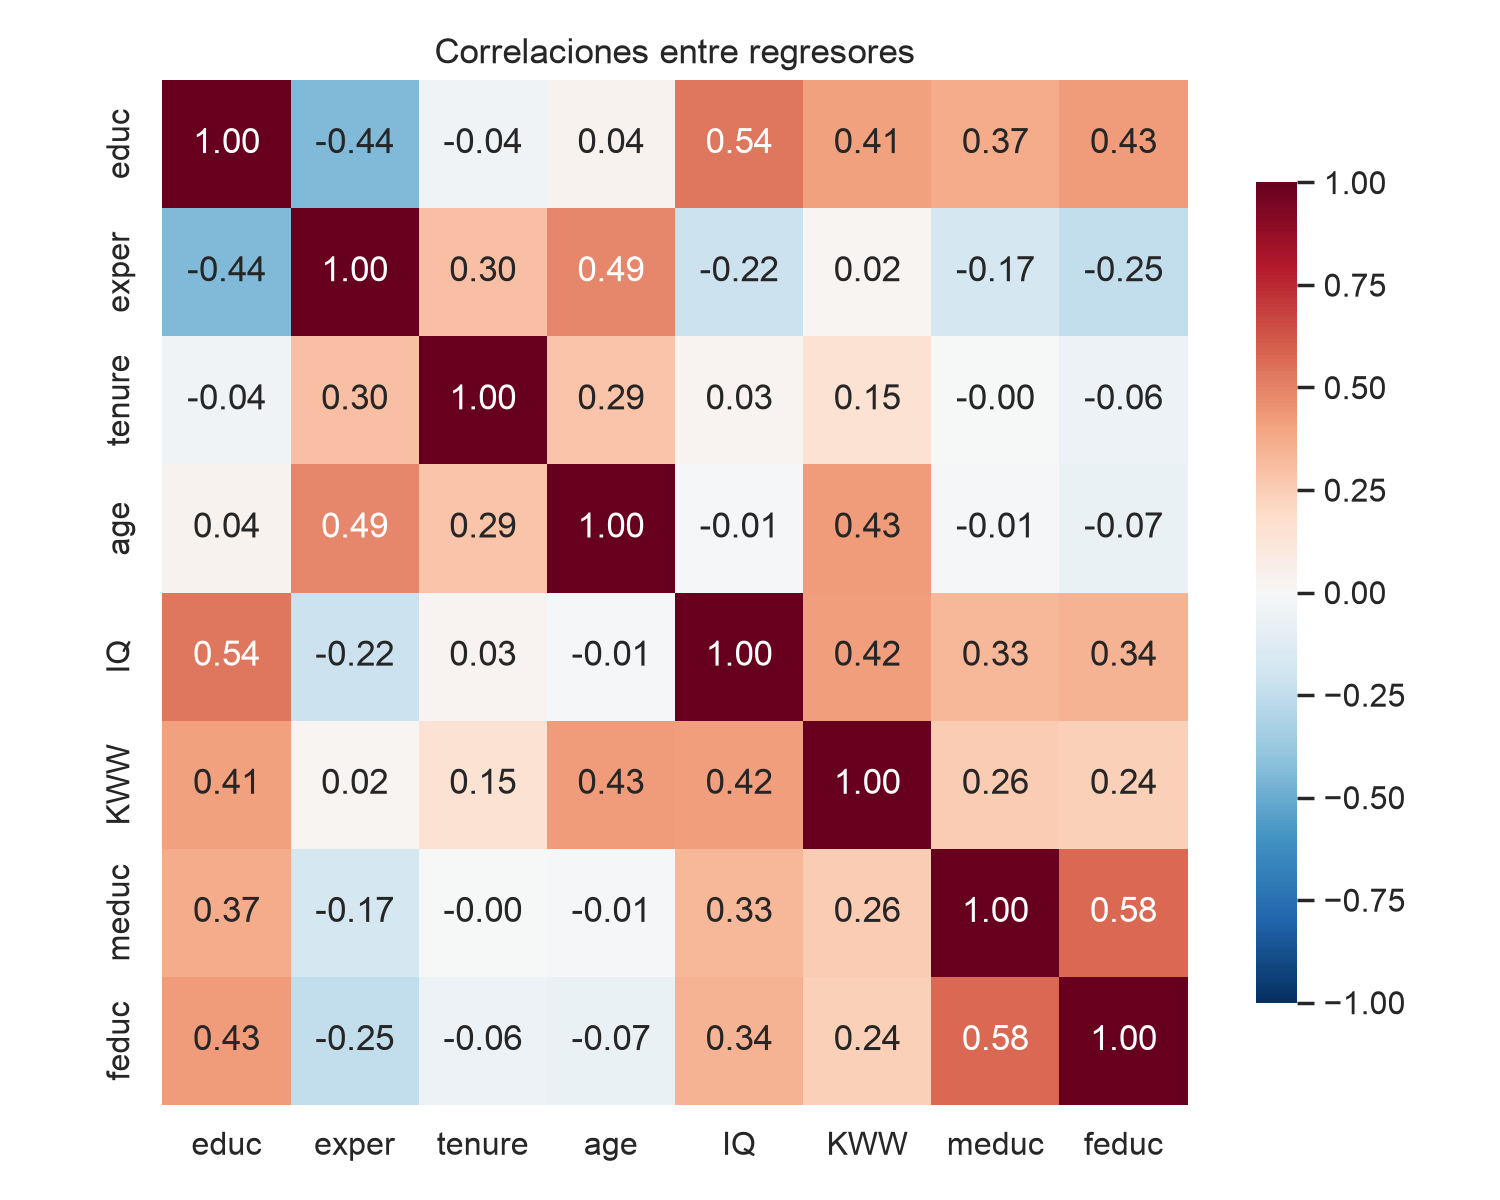
\includegraphics[width=\linewidth]{correlaciones}
\column{0.5\textwidth}\centering\scriptsize
$VIF_j=\dfrac{1}{1-R_j^2}$, \quad $Tol_j=1-R_j^2$
\vspace{0.3em}

\begin{tabular}{lrrr}
\toprule
Variable & VIF & Tol. & $R_j^2$ \\
\midrule
exper$^2$ & 24.01 & 0.042 & 0.958 \\
exper & 21.08 & 0.047 & 0.953 \\
educ & 2.17 & 0.461 & 0.539 \\
age & 2.07 & 0.483 & 0.517 \\
KWW & 1.74 & 0.575 & 0.425 \\
IQ & 1.73 & 0.577 & 0.423 \\
feduc & 1.69 & 0.590 & 0.410 \\
meduc & 1.58 & 0.631 & 0.369 \\
black & 1.23 & 0.815 & 0.185 \\
tenure & 1.16 & 0.863 & 0.137 \\
south & 1.10 & 0.913 & 0.087 \\
urban & 1.06 & 0.945 & 0.055 \\
married & 1.04 & 0.965 & 0.035 \\
\bottomrule
\end{tabular}\\[0.3em]
Klein: $R_j^2>R^2=0.264$ en 8 de 13 regresores.
\end{columns}
\end{frame}

\begin{frame}{Autovalores, número de condición y Farrar--Glauber}
\begin{itemize}
\item Regresoras estandarizadas: $\lambda_{\max}=3.273$, $\lambda_{\min}=0.0226$ $\Rightarrow$ $\kappa=\sqrt{\lambda_{\max}/\lambda_{\min}}=12.04$.
\item Columnas normalizadas con constante (Belsley--Kuh--Welsch): número de condición $=77.3$ $>30$ (severa).
\item Farrar--Glauber: $\chi^2=-\left[n-1-\frac{2k+5}{6}\right]\ln|R|$, con $|R|=0.0031$: $\chi^2=4140>\chi^2_{0.05;\,78}=99.6$ $\Rightarrow$ se rechaza ortogonalidad.
\item Síntoma clásico: $se(\hat\beta_{educ})$ sube de 0.0073 (base) a 0.0089 (completo).
\item \alert{MCO sigue siendo MELI}: la multicolinealidad no sesga, vuelve imprecisos los estimadores.
\end{itemize}
\end{frame}

\begin{frame}{Corrección: centrar, eliminar/combinar, PCA y Ridge}
\begin{columns}[T]
\column{0.5\textwidth}
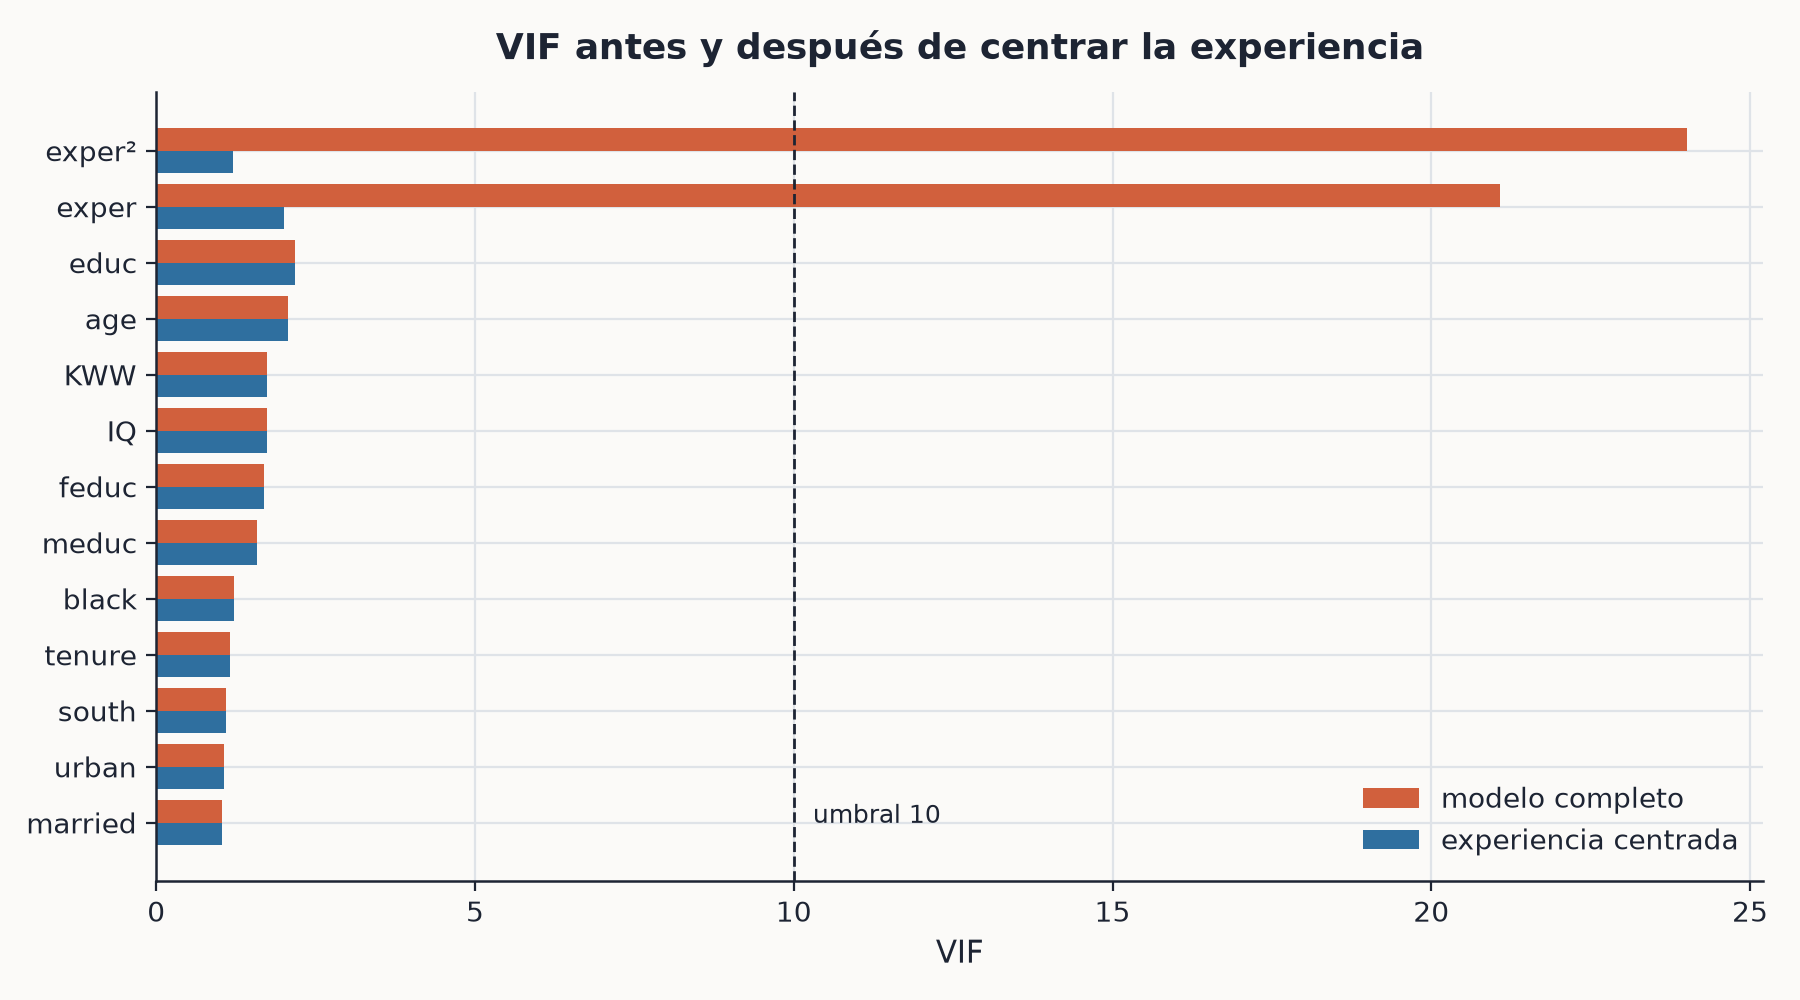
\includegraphics[width=\linewidth]{vif}
\column{0.5\textwidth}
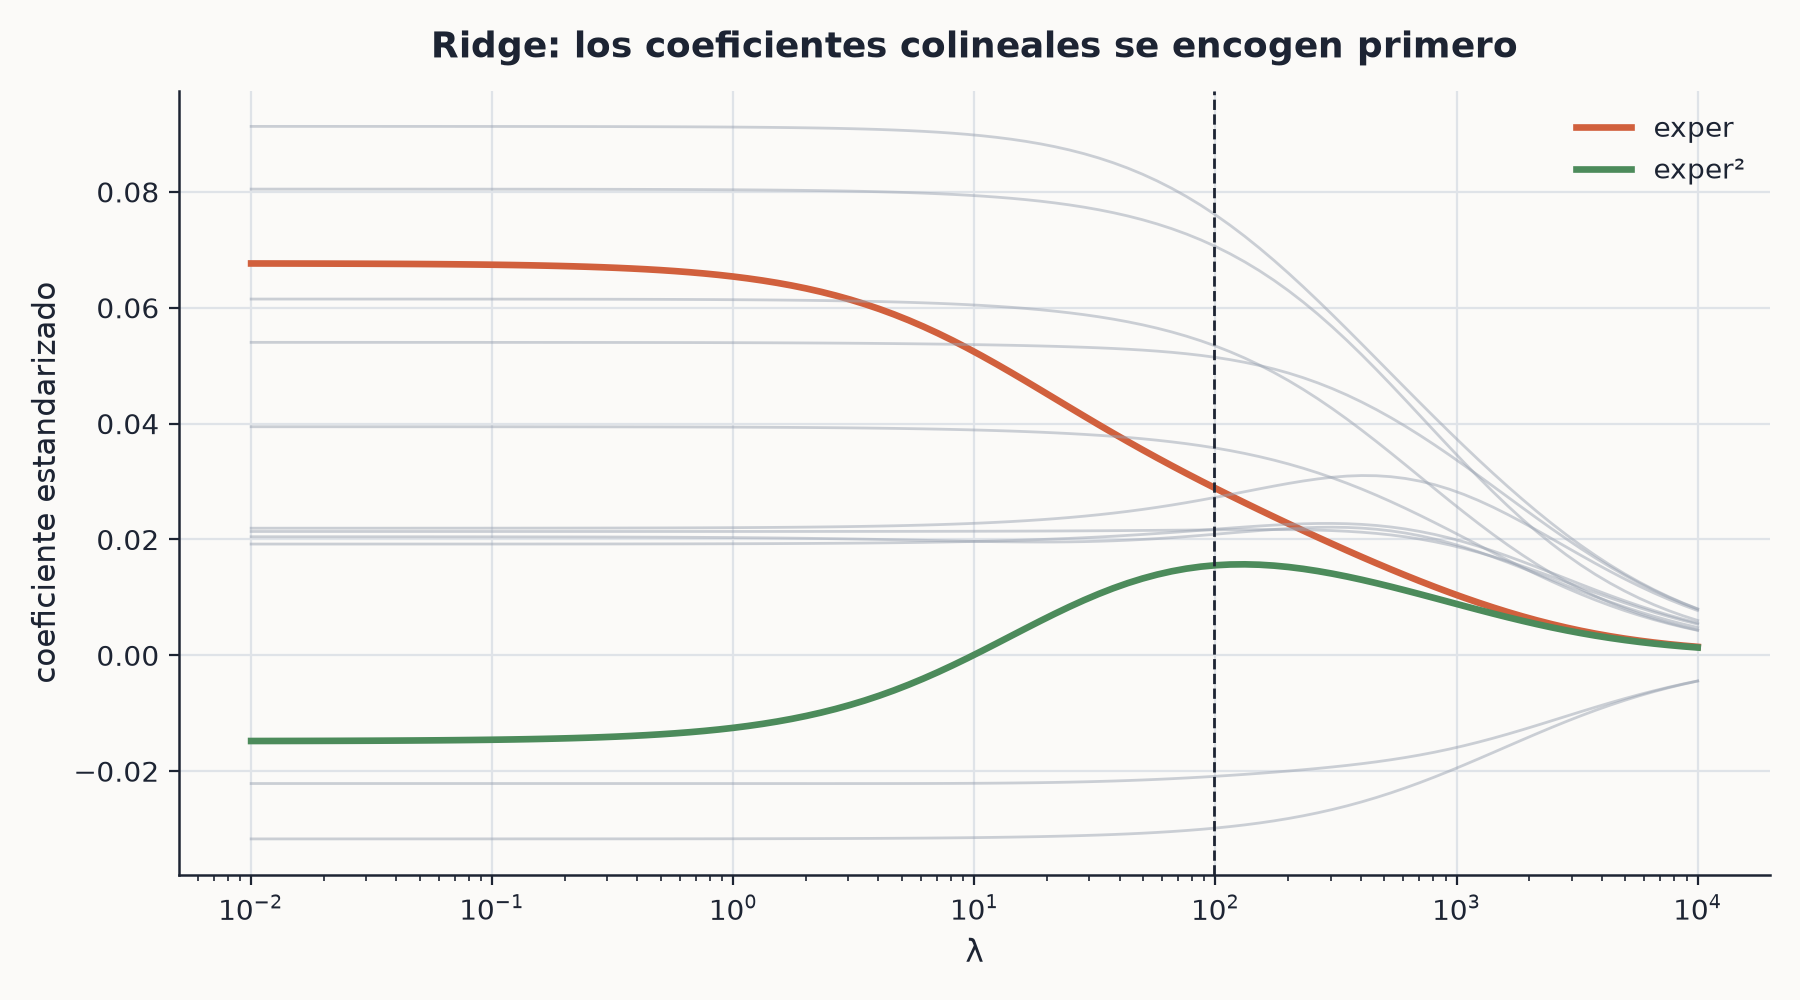
\includegraphics[width=\linewidth]{ridge}
\end{columns}
\small
\begin{itemize}
\item Centrar: $\mathrm{corr}(exper,exper^2)$ 0.975 $\to$ 0.054; VIF máx 24.0 $\to$ 2.17, mismo $R^2$.
\item Eliminar $age$ y promediar padres (prueba $F$ de $\beta_{meduc}=\beta_{feduc}$: $p=0.86$). PCA: CP1 $=52\%$ de la varianza. Ridge: $\lambda\approx 99$.
\end{itemize}
\end{frame}

\begin{frame}{Comparación de especificaciones}
\begin{columns}[T]
\column{0.60\textwidth}\centering\footnotesize\setlength{\tabcolsep}{4pt}
\begin{tabular}{lrrrrrr}
\toprule
Modelo & $\hat\beta_{educ}$ & ee & $\bar R^2$ & BIC & VIF máx & $k$ \\
\midrule
Base & 0.0783 & 0.0073 & 0.1373 & 709.8 & 20.4 & 3 \\
Completo & 0.0408 & 0.0089 & 0.2507 & 663.8 & 24.0 & 13 \\
Centrado & 0.0408 & 0.0089 & 0.2507 & 663.8 & 2.2 & 13 \\
Reducido & 0.0479 & 0.0082 & 0.2492 & 648.5 & 1.8 & 10 \\
PCA & 0.0468 & 0.0083 & 0.2507 & 641.6 & 1.9 & 9 \\
\bottomrule
\end{tabular}
\column{0.38\textwidth}
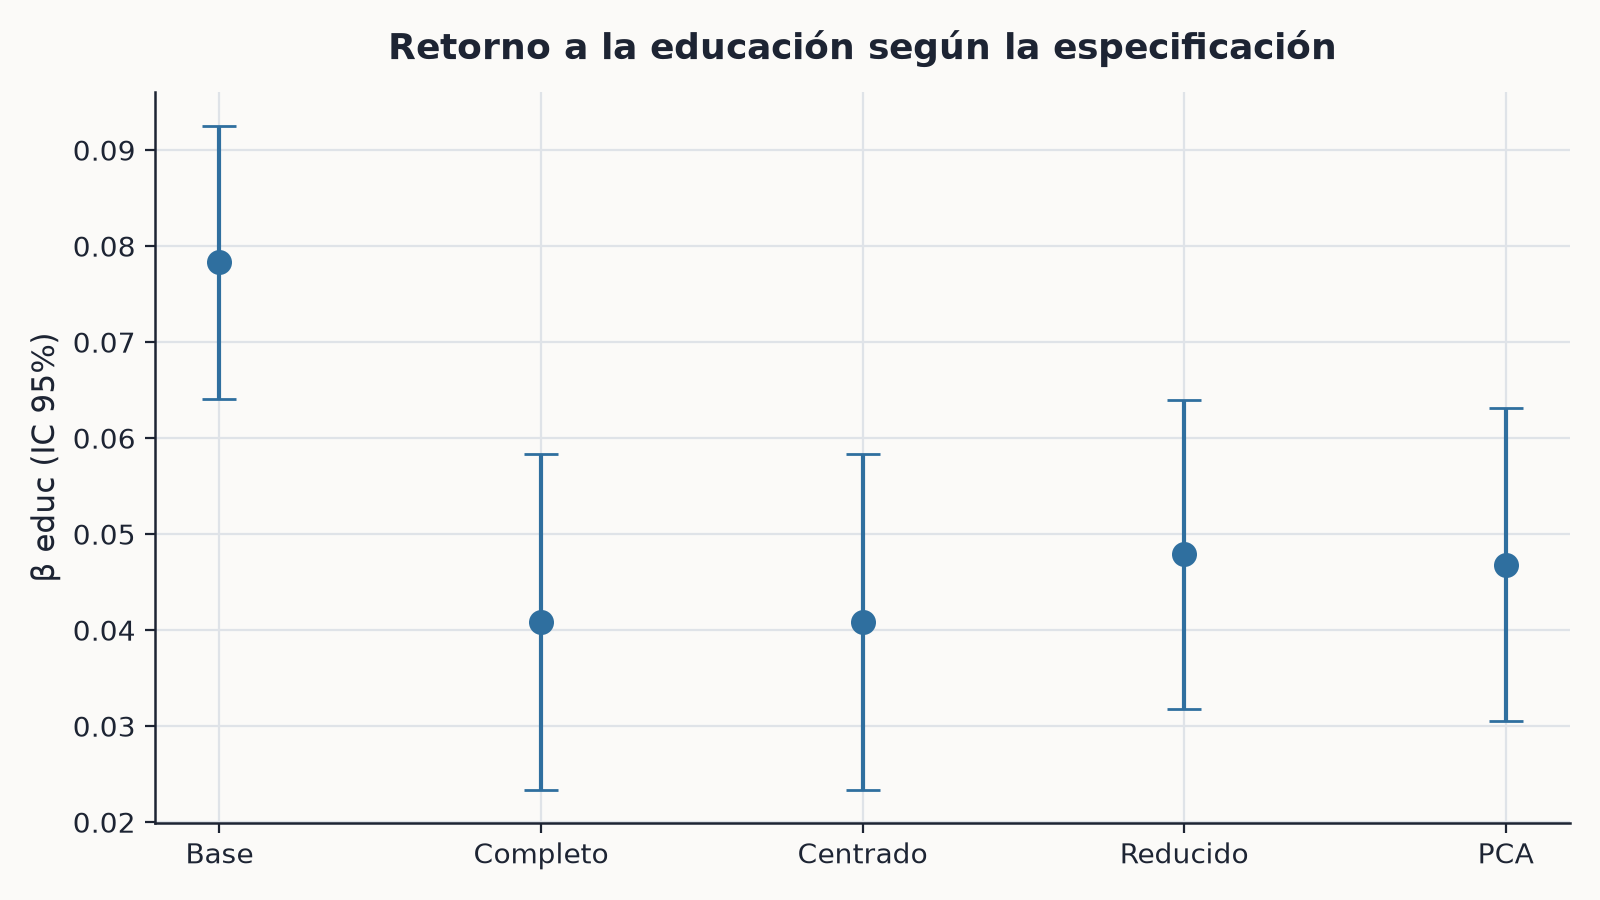
\includegraphics[width=\linewidth]{educ}
\end{columns}
\vspace{0.5em}
\small La caída de $\hat\beta_{educ}$ (base $\to$ completo) es \alert{sesgo por variable omitida} (habilidad); la multicolinealidad se nota en el error estándar.
\end{frame}

\section{MANOVA y 5.1--5.6}
\begin{frame}{MANOVA \quad\textbar\quad 5.1--5.2 Distribución de los residuos}
\begin{columns}[T]
\column{0.4\textwidth}\small
\textbf{MANOVA}: ¿difieren $(educ, IQ, KWW)$ entre el sur y el resto?
\begin{itemize}
\item Wilks $\Lambda=0.9737$
\item Pillai $=0.0263$
\item $F(3,718)=6.46$, $p<0.001$
\end{itemize}
MANOVA trata varias $Y$; \alert{no} diagnostica multicolinealidad (propiedad de las columnas de $X$).
\vspace{0.5em}

\textbf{Residuos}: sin curvatura ni abanico marcado; cola izquierda pesada; Cook máx $=0.050$.
\column{0.6\textwidth}
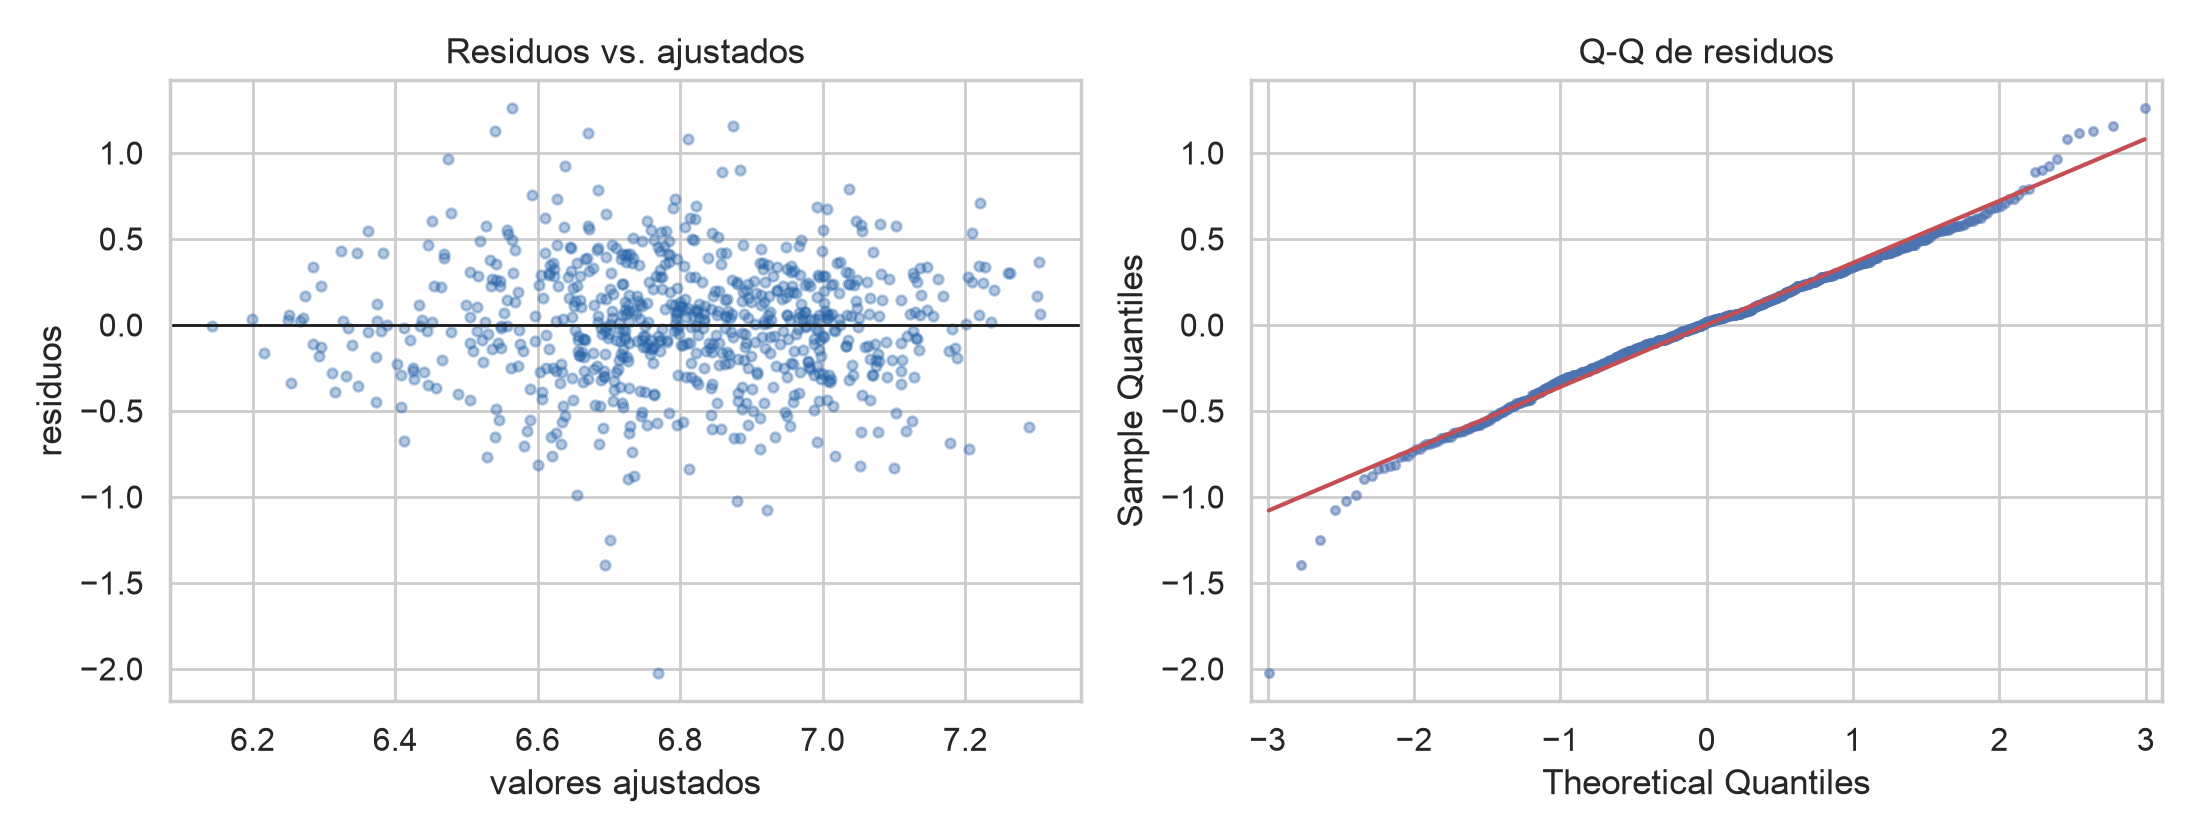
\includegraphics[width=\linewidth]{residuos}
\end{columns}
\end{frame}

\begin{frame}{5.3--5.6 Heteroscedasticidad: Breusch--Pagan paso a paso}
\begin{enumerate}
\item Estimar el modelo reducido por MCO y obtener $\hat\varepsilon_i$.
\item Regresión auxiliar de $\hat\varepsilon_i^2$ sobre las $q=10$ regresoras: $R^2_{aux}=0.0289$.
\item $LM=nR^2_{aux}=722\times0.0289=20.90$.
\item $LM>\chi^2_{0.05;\,10}=18.31$ ($p=0.022$) $\Rightarrow$ \alert{se rechaza homoscedasticidad}.
\end{enumerate}
\begin{itemize}
\item White: $p=0.27$ (pierde potencia por los muchos términos).
\item Errores HC0--HC3 casi iguales a los clásicos; WLS/FGLS: $\hat\beta_{educ}=0.0472$.
\item Los coeficientes MCO no cambian con errores robustos: sólo cambia su incertidumbre.
\end{itemize}
\end{frame}

\begin{frame}{Modelo final con errores robustos (HC1)}
\centering\scriptsize
\begin{tabular}{lrrrr}
\toprule
Variable & $\hat\beta$ & ee HC1 & $p$ & Efecto \% exacto \\
\midrule
educ & 0.0479 & 0.0087 & $<0.001$ & 4.91 \\
exper$_c$ & 0.0166 & 0.0038 & $<0.001$ & 1.67 \\
exper$_c^2$ & 0.0002 & 0.0007 & 0.747 & 0.02 \\
tenure & 0.0086 & 0.0030 & 0.004 & 0.86 \\
IQ & 0.0038 & 0.0011 & $<0.001$ & 0.39 \\
peduc & 0.0136 & 0.0053 & 0.010 & 1.37 \\
married & 0.2008 & 0.0431 & $<0.001$ & 22.24 \\
black & -0.0909 & 0.0480 & 0.058 & $-$8.69 \\
south & -0.0663 & 0.0324 & 0.041 & $-$6.41 \\
urban & 0.1842 & 0.0305 & $<0.001$ & 20.22 \\
\bottomrule
\end{tabular}
\vspace{0.5em}

\small $n=722$, $R^2=0.260$. Variable dependiente: $\ln w$. Bases: no casado, no negro, fuera del sur, rural.
\end{frame}

\section{5.7--5.13}
\begin{frame}{5.7--5.10 Autocorrelación: Durbin--Watson, Breusch--Godfrey y HAC}
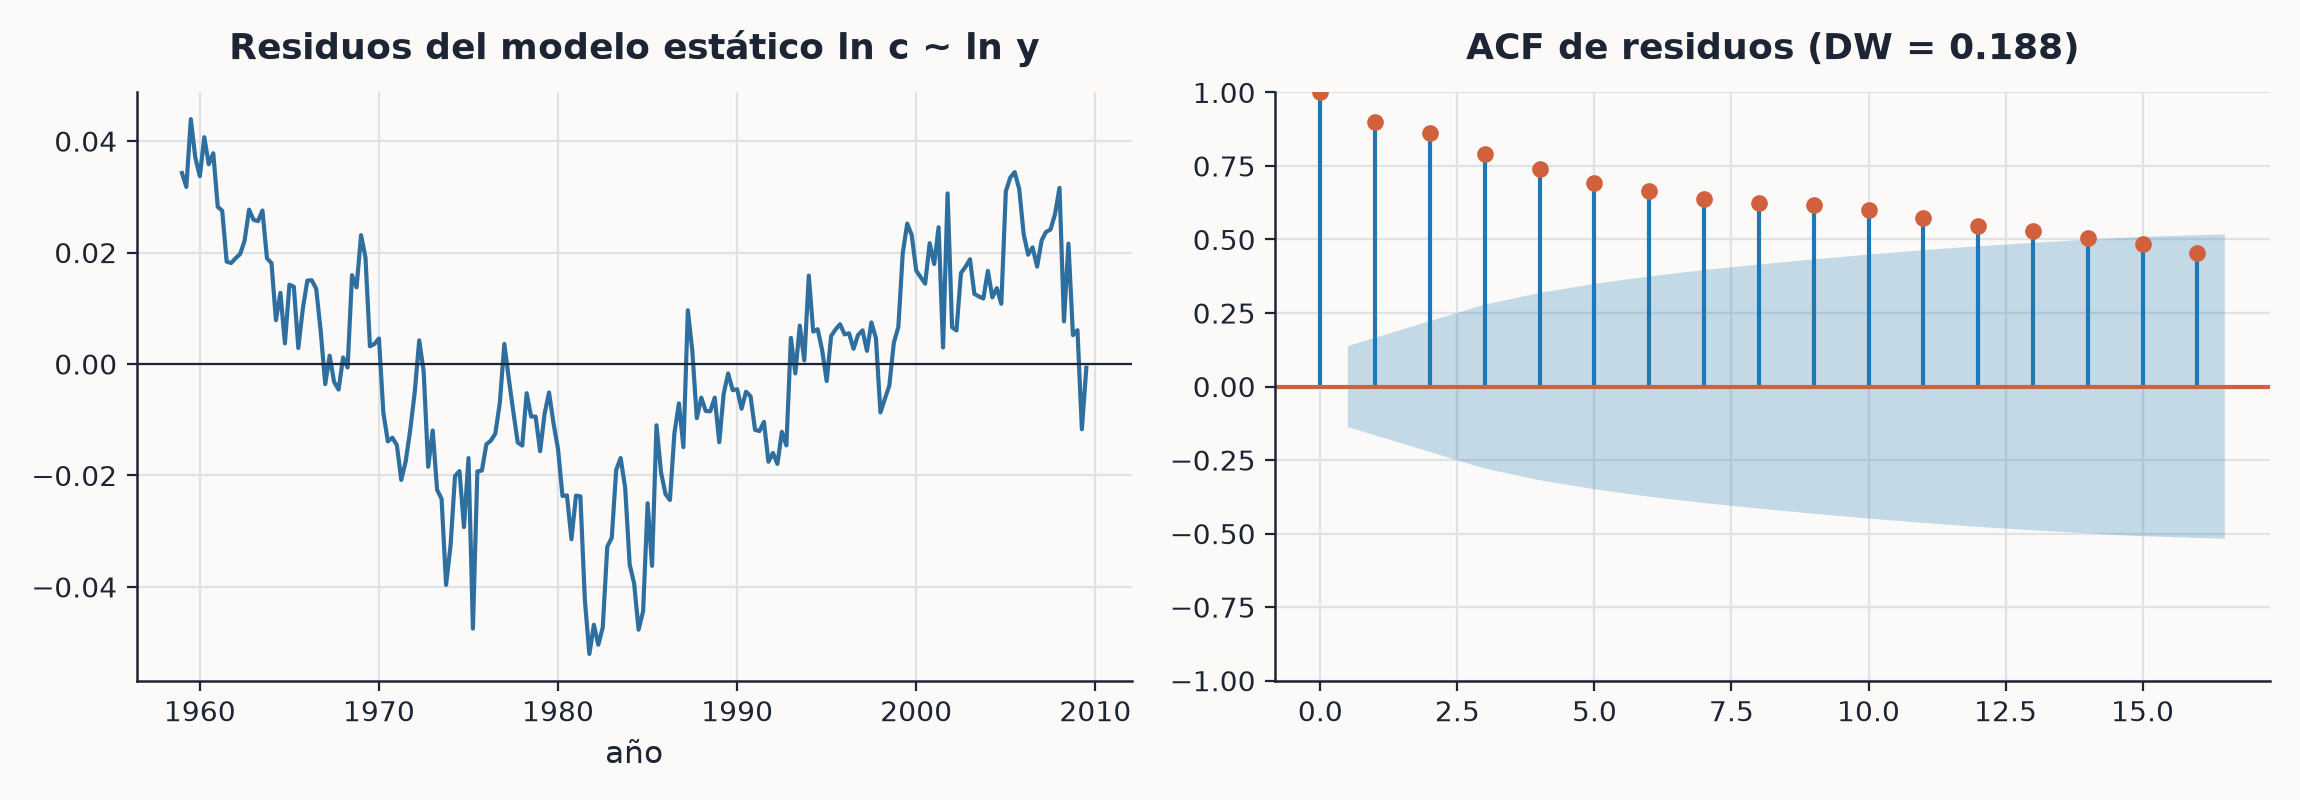
\includegraphics[width=\linewidth]{autocorrelacion}
\small
\begin{itemize}
\item wage2: DW $=1.864$ y $1.985$ al reordenar filas $\Rightarrow$ no aplica en corte transversal.
\item Consumo (macrodata, $n=203$), $\ln c=\alpha+\beta\ln y$: $R^2=0.9984$, DW $=0.188\approx2(1-\hat\rho)$ con $\hat\rho=0.906$; BG(4) $=167.8$.
\item $se$ HAC (Newey--West) $=0.0067$ vs clásico 0.0029: la inferencia clásica subestima la incertidumbre.
\end{itemize}
\end{frame}

\begin{frame}{5.11--5.12 Modelos dinámicos y rezagos}
\[\ln c_t=\alpha+\phi\ln c_{t-1}+\beta_0\ln y_t+\beta_1\ln y_{t-1}+u_t\]
\begin{columns}[T]
\column{0.5\textwidth}\small
\begin{itemize}
\item $\hat\phi=0.9539$ ($|\phi|<1$: estable)
\item $\hat\beta_0=0.3450$, \ $\hat\beta_1=$-$0.2989$
\item Largo plazo: $\dfrac{\beta_0+\beta_1}{1-\phi}=0.999\approx1$
\item $\mathrm{corr}(\ln y_t,\ln y_{t-1})=0.9998$: VIF $>3{,}000$ (\alert{multicolinealidad entre rezagos})
\item BG(4) aún rechaza: más dinámica o HAC
\end{itemize}
\column{0.5\textwidth}\centering\scriptsize
Rezagos distribuidos: $\Delta\ln c_t$ sobre $\Delta\ln y_{t-j}$\\[0.3em]
\begin{tabular}{rrrrr}
\toprule
$p$ & AIC & BIC & $\sum\beta$ & $\bar R^2$ \\
\midrule
0 & 379.6 & 386.2 & 0.342 & 0.190 \\
1 & 355.8 & 365.7 & 0.602 & 0.285 \\
2 & 356.0 & 369.2 & 0.660 & 0.288 \\
3 & 353.6 & 370.0 & 0.746 & 0.300 \\
4 & 355.6 & 375.3 & 0.744 & 0.296 \\
\bottomrule
\end{tabular}\\[0.3em]
\small BIC elige 1 rezago; AIC elige 3.
\end{columns}
\end{frame}

\begin{frame}{5.13 Jarque--Bera y resumen de diagnósticos}
\[JB=\frac{n}{6}\left(S^2+\frac{(K-3)^2}{4}\right)=\frac{722}{6}\left((-0.303)^2+\frac{(4.849-3)^2}{4}\right)=113.9>\chi^2_{0.05;2}=5.99\]
\centering\small
\begin{tabular}{llll}
\toprule
Prueba & Estadístico & $p$ & Conclusión (5\%) \\
\midrule
Breusch--Pagan & LM $=$ 20.90 & 0.022 & Rechaza homoscedasticidad \\
White & LM $=$ 66.10 & 0.275 & No rechaza \\
RESET & F $=$ 0.846 & 0.430 & No rechaza \\
Jarque--Bera & JB $=$ 113.9 & $<0.001$ & Rechaza normalidad \\
DW (consumo) & DW $=$ 0.188 & -- & $\rho>0$ fuerte \\
BG(4) (consumo) & LM $=$ 167.8 & $<0.001$ & Autocorrelación \\
BG(4) (ARDL) & LM $=$ 24.3 & $<0.001$ & Aún rechaza \\
\bottomrule
\end{tabular}
\vspace{0.4em}

\raggedright Rechazar normalidad con $n=722$ no implica sesgo: la inferencia es válida asintóticamente.
\end{frame}

\section{Cierre}
\begin{frame}{Inferencia vs predicción}
\begin{columns}[T]
\column{0.5\textwidth}\centering
\begin{tabular}{lrr}
\toprule
Modelo & $R^2$ prueba & RMSE \\
\midrule
Base & 0.0405 & 0.3705 \\
Completo & 0.2239 & 0.3332 \\
Reducido & 0.2215 & 0.3338 \\
Ridge & 0.2504 & 0.3275 \\
\bottomrule
\end{tabular}
\column{0.5\textwidth}
\begin{itemize}
\item Completo $\approx$ reducido fuera de muestra.
\item La multicolinealidad daña la \alert{interpretación}, no la predicción.
\item Ridge: menor RMSE a cambio de sesgo (no reporta $p$-values).
\end{itemize}
\end{columns}
\end{frame}

\begin{frame}{Conclusiones}
\begin{enumerate}
\item Retorno a la educación robusto: 5.9\% (simple) $\to\approx$4.8\% con habilidad (sesgo por variable omitida).
\item Perfecta: no hay MCO único. Imperfecta: MCO sigue siendo MELI, pero las varianzas se inflan.
\item VIF, tolerancia, Klein, autovalores, número de condición y Farrar--Glauber señalan $exper$, $exper^2$ y $age$.
\item La $F$ conjunta revela lo que las $t$ individuales no pueden.
\item Centrar, combinar, PCA o Ridge corrigen sin perder ajuste.
\item Heteroscedasticidad leve (HC1); no normalidad irrelevante con $n$ grande; en series de tiempo, dinámica o HAC.
\item La misma lección aparece en hedónicos, finanzas y rezagos.
\end{enumerate}
\end{frame}

\begin{frame}{Referencias}
\small
\begin{itemize}
\item Belsley, Kuh y Welsch (1980). \textit{Regression Diagnostics}. Wiley.
\item Davidson y MacKinnon (1981). \textit{Econometrica}, 49(3), 781--793.
\item Farrar y Glauber (1967). \textit{Review of Economics and Statistics}, 49(1), 92--107.
\item Galindo, C. (2026). Notas de regresión lineal, pruebas $t$ y $F$, inferencia y diagnóstico. Universidad Panamericana.
\item Koenker y Bassett (1978). Regression quantiles. \textit{Econometrica}, 46(1), 33--50.
\item Mincer, J. (1974). \textit{Schooling, Experience, and Earnings}. NBER.
\item Wooldridge, J. M. (2020). \textit{Introducción a la econometría} (7.\textsuperscript{a} ed.). Cengage.
\end{itemize}
\end{frame}

\end{document}
